\documentclass[11pt]{article}

\usepackage[margin=1in]{geometry}
\usepackage{amsmath,amssymb,amsfonts}
\usepackage{microtype}
\usepackage{graphicx}
\usepackage{booktabs}
\usepackage{array}
\usepackage{tikz}
\usetikzlibrary{positioning,arrows.meta,fit,calc}
\usepackage{subcaption}
\usepackage[numbers,sort&compress]{natbib}
\usepackage[hidelinks]{hyperref}
\usepackage[nameinlink,capitalize,noabbrev]{cleveref}

\title{Phase-Associative Memory: Attention-Free Sequence Modeling via Complex Matrix States}
\author{%
  Gowrav Vishwakarma\thanks{Code: \url{https://github.com/gowrav-vishwakarma/qllm2}} \\
  Independent Researcher, India \\[6pt]
  Christopher J. Agostino \\
  NPC Worldwide, Bloomington, Indiana 47403, USA
}
\date{March 2026}

\newcommand{\Complex}{\mathbb{C}}
\newcommand{\Repart}{\operatorname{Re}}
\newcommand{\softmax}{\operatorname{softmax}}
\newcommand{\concat}{\operatorname{concat}}

\begin{document}
\maketitle

\begin{abstract}
Recent work in quantum cognition has demonstrated that semantic interpretation---in both humans and large language models---exhibits non-classical contextuality, producing correlations that violate Bell-type inequalities. If the structure of meaning is genuinely non-classical, then architectures whose native operations are complex-valued superposition and phase interference may be better suited to modeling language than those grounded in classical probability. We test this hypothesis by constructing Phase-Associative Memory (PAM), a recurrent sequence model that operates entirely in complex-valued space. Each PAM head maintains a matrix state $S_t \in \Complex^{d \times d}$, updated via outer products of complex key--value pairs and retrieved via conjugate inner products $K_t^* \cdot \tilde{Q}_t$, where phase alignment between query and stored key determines retrieval strength through constructive and destructive interference---without softmax normalization. A Gated State Protection mechanism allows selective freezing of state dimensions. PAM admits a dual computational form: $O(T^2)$ parallel training equivalent to its $O(1)$-per-token recurrent inference, requiring no KV cache.

We evaluate PAM as the core sequence layer in a 100M-parameter language model on WikiText-103, achieving validation perplexity \textbf{29.95}---within $\sim$10\% of a matched transformer baseline (\textbf{27.08}) trained under identical conditions. That a fundamentally different mathematical structure---complex matrix states with phase-geometric retrieval rather than softmax attention over real-valued representations---reaches competitive performance at this scale is itself a finding: the algebraic structure of complex interference is sufficient for sequence modeling, and the $\sim$10\% gap was achieved without custom kernels and with 4$\times$ arithmetic overhead from complex computation. We discuss what this result implies about the structure of the problem being modeled and what remains open. \textbf{Code:} \url{https://github.com/gowrav-vishwakarma/qllm2}.
\end{abstract}

\section{Introduction}
\label{sec:intro}

The question of what mathematical structure is appropriate for modeling natural language is usually treated as settled: real-valued vector spaces, with softmax-normalized dot products to route information between positions. The transformer architecture~\cite{vaswani2017attention} embodies this choice and has been spectacularly successful. But the question is worth reopening, because there is growing evidence that the structure of semantic interpretation is not classical in a precise, testable sense.

Experiments in quantum cognition have demonstrated that human semantic processing produces correlations that violate Bell-type inequalities~\cite{busemeyer2012quantum,bruza2023contextuality}---the same inequalities whose violation in physics established that measured quantities are not pre-determined but constituted in the act of measurement. Recent work has extended these tests to large language models, finding violations of the CHSH inequality ($|S| > 2$) across models spanning four orders of magnitude in parameter count, with the character of contextuality---as measured by the interquartile range of the $|S|$ distribution---completely orthogonal to standard benchmarks~\cite{agostino2025quantum,agostino2026production}. Using Kolmogorov complexity, it has been shown that the informational burden of disambiguating a semantic expression grows superlinearly with its complexity, making the recovery of a single intended meaning computationally intractable for expressions of even moderate depth~\cite{agostino2025quantum}. If meaning is not a fixed property of an expression but is produced in the encounter between expression and interpreter, then the formalism used to model that process matters: classical probability theory, which presupposes well-defined values prior to observation, may be the wrong starting point.

This paper takes that possibility seriously by constructing a language model whose native operations are complex-valued superposition and phase interference rather than real-valued dot products and softmax normalization. Phase-Associative Memory (PAM) maintains a complex matrix state $S_t \in \Complex^{d \times d}$ per head, accumulates associations via outer products of complex key--value pairs, and retrieves via conjugate inner products $K_t^* \cdot \tilde{Q}_t$ whose magnitude depends on phase alignment---constructive interference amplifies recall, destructive interference suppresses it. The entire model, from embedding through retrieval to output projection, operates in complex space with phase-preserving primitives end to end. There is no softmax, no KV cache, and inference cost per token is $O(1)$ in sequence length.

Structurally, PAM belongs to the family of decay-weighted linear attention models---fast weight programmers~\cite{schmidhuber1992learning,schlag2021linear} with matrix-valued state---that includes RetNet~\cite{sun2023retentive}, GLA~\cite{yang2024gated}, DeltaNet~\cite{yang2024deltanet}, and mLSTM~\cite{beck2024xlstm}. What distinguishes PAM is that lifting this structure to complex space introduces phase interference as a retrieval mechanism, providing a geometric selectivity---based on the alignment of phases between query and stored key---that has no analogue in real-valued matrix states. This is not a superficial notational change; it means that PAM's retrieval quality depends on a degree of freedom (phase) that real-valued models do not possess.

PAM emerged through a multi-stage research process. Early versions (V4) introduced tokens in complex phase space but passed them through real-valued nonlinearities that destroyed phase information. V5 corrected this with phase-preserving primitives (modReLU, ComplexGatedUnit, ComplexNorm) and showed that mathematical consistency materially improved results. V6 built a multi-timescale complex SSM backbone, but initial experiments with vector-state models showed that associative capacity was limited by destructive interference when multiple bindings accumulated in a single vector---the classical $O(1/\sqrt{n})$ degradation of holographic reduced representations~\cite{plate1995holographic}. PAM solves this by upgrading the state from a vector ($\Complex^d$) to a matrix ($\Complex^{d \times d}$), providing $O(d^2)$ associative capacity per head. The reported configuration (\textbf{medium-pam-v3}) interleaves channel mixing and PAM in each of 16 blocks with complex RoPE on queries and keys for relative position encoding.

At $\sim$100M parameters on WikiText-103, PAM achieves validation perplexity \textbf{29.95}. A matched transformer baseline ($\sim$100M parameters, identical data, tokenizer, sequence length, and training budget) reaches \textbf{27.08}---a gap of $\sim$10\%. We do not claim that PAM matches or exceeds transformers. What we do claim is that the gap is surprisingly small given the differences: PAM uses a fundamentally different mathematical structure (complex matrix states with phase-geometric retrieval), was implemented in pure PyTorch with no custom CUDA kernels, and operates with 4$\times$ the arithmetic overhead of real-valued computation. That complex-valued phase interference is sufficient for competitive language modeling at this scale is itself a result, and one whose implications extend beyond the engineering question of whether PAM can close the remaining gap.

\section{Background}
\label{sec:related}

The development of efficient alternatives to softmax attention has, over the past several years, converged on a specific mathematical structure: a matrix-valued state that accumulates outer products of keys and values, with some form of decay or gating to manage capacity, and retrieval via matrix--vector product with a query. This structure---the fast weight programmer~\cite{schmidhuber1992learning}, rediscovered as linear attention~\cite{katharopoulos2020transformers} and formalized as such by Schlag et al.~\cite{schlag2021linear}---appears to be a natural design point, arrived at independently from the linear algebra side (RetNet~\cite{sun2023retentive}, GLA~\cite{yang2024gated}, DeltaNet~\cite{yang2024deltanet}), the state-space model side (Mamba-2~\cite{dao2024transformers}), and the LSTM side (mLSTM~\cite{beck2024xlstm}). The convergence is informative: it suggests that this is not merely one possible architecture but something closer to a minimal sufficient structure for sequence modeling with fixed-size state.

PAM operates within this structure but makes a specific choice that none of its real-valued relatives make: the state, keys, values, and queries are all complex-valued, and retrieval uses the conjugate inner product $K^* \cdot Q$ rather than the standard inner product $K \cdot Q$. This is not an incremental modification. The conjugate inner product measures phase alignment---a geometric property of complex vectors with no real-valued analogue---and produces constructive or destructive interference depending on that alignment. The question this paper addresses is whether this additional degree of freedom matters for language modeling, and what it might mean if it does.

\subsection{From attention to matrix-state recurrence}
The transformer~\cite{vaswani2017attention} computes attention as $\softmax(QK^\top / \sqrt{d})V$, where queries, keys, and values are linear projections of the input. This is powerful but costs $O(T^2)$ per layer and requires a KV cache that grows linearly with sequence length during inference. Rotary position embeddings (RoPE; \citealt{su2024roformer}) encode relative position in the $QK^\top$ product by position-dependent rotations in embedding space; PAM applies an analogous \textbf{complex} phase rotation to $Q$ and $K$ only (\cref{sec:pam-rope}). Numerous efficiency variants exist (sparse attention, linear attention, sliding window), but the core mechanism remains fundamentally quadratic.

\subsection{The convergence on matrix-state recurrence}
Removing softmax from attention yields a recurrent form with matrix state $S_t = S_{t-1} + V_t K_t^\top$---a fast weight programmer~\cite{schmidhuber1992learning,schlag2021linear} that accumulates associations via outer products and retrieves via matrix--vector product. The subsequent history of the field can be read as a series of refinements to this basic structure: RetNet~\cite{sun2023retentive} adds exponential decay; GLA~\cite{yang2024gated} introduces data-dependent matrix gating; DeltaNet~\cite{yang2024deltanet} replaces additive accumulation with a delta rule that can overwrite old associations; GateLoop~\cite{katsch2024gateloop} uses fully complex-valued data-dependent gates; HGRN2~\cite{qin2024hgrn2} constructs matrix states via outer-product state expansion. From the state-space model side, the Linear Recurrent Unit~\cite{orvieto2023resurrecting} showed that complex-valued diagonal recurrences with magnitude constraints are critical for stable long-range modeling, Mamba~\cite{gu2023mamba} introduced input-dependent selection, Griffin~\cite{de2024griffin} validated gated linear recurrence at scale, and Mamba-2~\cite{dao2024transformers} proved the formal duality between structured SSMs and linear attention. From the LSTM side, mLSTM~\cite{beck2024xlstm} independently arrives at the same matrix-state recurrence ($C_t = f_t C_{t-1} + i_t v_t k_t^\top$). RWKV~\cite{peng2023rwkv,peng2024eagle} demonstrated this family at scale up to 14B parameters.

That three distinct research lineages---linear attention, state-space models, and gated recurrent networks---converge on the same mathematical object suggests it is not arbitrary. The matrix state with outer-product updates and decay-weighted retrieval appears to be a minimal sufficient structure for fixed-size sequence modeling. PAM's update $S_t = \gamma_t S_{t-1} + V_t \otimes K_t^*$ belongs to this family, but the conjugate in $K_t^*$ and the complex-valued state introduce a qualitative difference: retrieval depends on phase alignment, a geometric degree of freedom absent in all real-valued members of this convergent family. The question is whether that degree of freedom matters, and what it would mean if it does.

\subsection{Phase as a representational primitive}
A classical result in signal processing is that phase carries more structural information than magnitude: swapping the phase spectra of two images produces a result resembling the image whose phase was kept, not whose magnitude was kept~\cite{oppenheim1981importance}. This asymmetry is well-known in signal processing but has received remarkably little attention in the design of language models, where representations are almost universally real-valued.

Complex-valued neural networks have been studied for decades~\cite{hirose2012complex}, with key ingredients including phase-preserving activations like modReLU~\cite{arjovsky2016unitary} and unitary recurrent dynamics~\cite{trabelsi2018deep}. Danihelka et al.~\cite{danihelka2016associative} combined holographic reduced representations~\cite{plate1995holographic} with LSTM using complex-valued cell states, demonstrating that complex associative memory can function within a recurrent architecture---the most direct precursor to PAM. From the associative memory perspective, Ramsauer et al.~\cite{ramsauer2021hopfield} showed that softmax attention implements a modern Hopfield network, an exponential associative memory; linear attention removes the exponential, yielding a linear associative memory~\cite{schlag2021linear}. PAM equips this linear memory with a complex-valued similarity metric---the conjugate inner product---that provides phase-based selectivity.

The motivation for taking phase seriously in language modeling comes from an unexpected direction. Experiments in quantum cognition~\cite{busemeyer2012quantum,bruza2023contextuality} have demonstrated that human semantic processing exhibits non-classical contextuality, producing correlations that violate Bell-type (CHSH) inequalities. Recent work~\cite{agostino2025quantum,agostino2026production} extended these tests to large language models, finding violations across models spanning four orders of magnitude in scale, with the character of contextuality---as measured by the $|S|$ distribution---completely orthogonal to standard benchmarks. The informational burden of disambiguating a semantic expression was shown to grow superlinearly with complexity~\cite{agostino2025quantum}, suggesting that the recovery of a single determinate meaning is computationally intractable and that the classical assumption of pre-existing, context-independent meanings is inadequate as a modeling foundation.

If the structure of semantic interpretation is genuinely non-classical---if meanings are produced rather than retrieved, and if this production involves interference between possible interpretations---then the formalism used to model it matters. Classical probability assigns positive real weights that sum to one; complex amplitudes can interfere constructively and destructively, and their squared magnitudes yield probabilities only upon measurement. PAM does not implement quantum mechanics, but it implements the same algebraic structure: complex-valued superposition, phase-dependent retrieval, and interference as an intrinsic property of the inner product rather than a learned behavior. The question is whether this structural consonance is incidental or whether it reflects something about the problem being modeled.\footnote{This is not a claim about the physical substrate. LLMs run on silicon, not quantum hardware. The claim is structural: the algebraic properties of complex inner products---specifically, the capacity for constructive and destructive interference based on phase alignment---may be better matched to the non-classical correlational structure of semantic interpretation than the positive-real-valued operations of standard architectures. The same algebraic structure can be implemented on classical hardware, as PAM demonstrates.}

\section{Method}
\label{sec:method}

\subsection{Overview}
The \textbf{medium-pam-v3} backbone interleaves channel mixing and sequence mixing in each block (preset \texttt{interleave\_pam=True}). The full model is:
\begin{verbatim}
Tokens -> ComplexEmbed -> ComplexNorm
  -> [ ComplexGatedUnit + residual
       -> PhaseAssociativeLayer + residual ] x 16 blocks
  -> ComplexLinear -> ComplexNorm -> TiedComplexLMHead
\end{verbatim}
An earlier \textbf{sequential} layout (\texttt{medium-pam}) instead ran \texttt{[CGU + residual] x 16} followed by \texttt{[PAM + residual] x 16}; \cref{sec:main-result} reports both.

All operations in the main signal path are complex-valued and phase-preserving. Control signals (gates, decay parameters) may use real-valued projections over magnitude features, but the primary data path never converts complex representations to real-valued intermediate forms.

\subsection{Phase-preserving primitives}
These primitives, inherited from V5, form the algebraic foundation:

\paragraph{Complex representation.} All tensors have shape \texttt{[..., dim, 2]}, where the last dimension holds (real, imaginary) components. This is a concrete implementation of $\Complex^{\text{dim}}$.

\paragraph{Complex linear map.} Given weight matrices $W_r, W_i \in \mathbb{R}^{m \times n}$, the complex linear map computes:
\begin{equation}
  y_r = W_r x_r - W_i x_i, \quad y_i = W_i x_r + W_r x_i .
\end{equation}
This is standard complex matrix multiplication. Conceptually it corresponds to four real matrix multiplies; the \textbf{training implementation} packs them into a \textbf{single block-real GEMM} (max float32 error $\sim 4\times 10^{-6}$ vs.\ the unpacked form in our checks), reducing kernel launches without changing the math.

\paragraph{modReLU.} A phase-preserving activation that thresholds magnitude while leaving phase untouched:
\begin{equation}
  \operatorname{modReLU}(z) = \operatorname{ReLU}(|z| + b) \cdot \frac{z}{|z|}
\end{equation}
where $b$ is a learned bias. This replaces GELU/ReLU, which would destroy phase information.

\paragraph{ComplexNorm.} RMS normalization applied to magnitudes, with phase preserved:
\begin{equation}
  \operatorname{ComplexNorm}(z) = s \cdot \frac{|z|}{\operatorname{RMS}(|z|)} \cdot \frac{z}{|z|}
\end{equation}
where $s$ is a learned scale parameter.

\paragraph{ComplexGatedUnit (CGU).} A SwiGLU-style gating block in complex space. The gate magnitude $\sigma(|W_g z|)$ controls how much signal passes, while the gate phase controls what rotation is applied. An up-projection through modReLU provides the nonlinearity:
\begin{equation}
  \operatorname{CGU}(z) = W_{\text{down}}\bigl( \mathrm{gate}_{\mathrm{phase}} \odot \operatorname{modReLU}(W_{\text{up}} z) \cdot \sigma(|W_g z|) \bigr)
\end{equation}

\subsection{Blocks (interleaved CGU and PAM)}
\label{sec:blocks}
Each of 16 blocks applies \textbf{channel mixing} then \textbf{sequence mixing} with residual connections and learned scaling:
\begin{align}
  \tilde{z}^{(l)} &= z^{(l-1)} + \alpha^{(l)}_{\text{CGU}} \cdot \text{CGU}_l(\operatorname{ComplexNorm}(z^{(l-1)})), \\
  z^{(l)} &= \tilde{z}^{(l)} + \alpha^{(l)}_{\text{PAM}} \cdot \text{PAM}_l(\operatorname{ComplexNorm}(\tilde{z}^{(l)}))
\end{align}
where $\alpha^{(l)}_{\text{CGU}}$ is initialized to $1.0$ and $\alpha^{(l)}_{\text{PAM}}$ to $0.1$. Each CGU uses expansion factor 3 (hidden dimension $3 \times 384 = 1152$). Dropout is applied during training.

\subsection{Phase-Associative Memory (PAM)}
\label{sec:pam}
PAM is the core contribution. It replaces both the recurrent backbone (SSM) and the attention mechanism with a single module.

\subsubsection{State representation}
Each PAM head $h$ maintains a complex matrix state $S_t^{(h)} \in \Complex^{d \times d}$, where $d$ is the head dimension. With $H$ heads and head dimension $d$, the total state capacity is $H \times d^2$ complex values. In our configuration ($H = 6$, $d = 64$), this is $6 \times 64^2 = 24{,}576$ complex values per layer.

\subsubsection{Projections and fused QKV}
The input $x_t \in \Complex^D$ (where $D = 384$) is projected into queries, keys, and values. In \textbf{medium-pam-v3}, a \textbf{single} complex linear map produces a vector of length $3Hd$, which is reshaped into $Q_t, K_t, V_t$; this is equivalent to three separate maps and does not change the parameter count.
\begin{equation}
  [Q_t; K_t; V_t] = W_{\text{QKV}} x_t \quad \Rightarrow \quad Q_t, K_t, V_t \in \Complex^{H \times d} .
\end{equation}

\subsubsection{Complex RoPE on Q and K}
\label{sec:pam-rope}
We apply \textbf{complex RoPE} to $Q$ and $K$ only (not $V$, not the residual stream). For each head dimension and position $m$, $Q_{m}$ and $K_{m}$ are multiplied element-wise by precomputed \textbf{unit-magnitude} complex factors $e^{i m \theta}$ (frequencies $\theta$ fixed by dimension, as in standard RoPE). Thus $|Q|, |K|$ are unchanged and phase encodes absolute position; in products $K_i^* \cdot \tilde{Q}_t$, dependence on $(m{-}n)$ yields \textbf{relative} position structure. RoPE is applied \textbf{before} forming training-time $Q K^{*\top}$ and before each recurrent inference step (with an explicit step offset during generation).

\subsubsection{Scaled query for retrieval}
\label{sec:scaled-query}
Following the attention scaling convention, we define the \textbf{scaled query}
\begin{equation}
  \tilde{Q}_t := \frac{1}{\sqrt{d}}\, Q_t .
\end{equation}
All retrieval dot products in \cref{sec:pam-retrieval,sec:dual-form,sec:recurrent-form} use $\tilde{Q}_t$ (implemented by scaling $Q$ before the complex bilinear form). Unscaled $Q_t$ still appears in projections and RoPE; only the score and matrix--vector product use $\tilde{Q}_t$.

\subsubsection{Data-dependent decay}
The decay rate $\gamma_t$ controls how quickly the state forgets. It is computed from the input:
\begin{equation}
  dt_t = \operatorname{softplus}(W_{dt} \cdot \concat(x_{t,r}, x_{t,i}) + b_{dt})
\end{equation}
where $W_{dt} \in \mathbb{R}^{H \times 2D}$ projects the concatenated real and imaginary parts to one scalar per head, and $b_{dt}$ is initialized to $-4.0$ (yielding slow initial decay).

\subsubsection{Gated State Protection (GSP)}
GSP adds a learned protect gate $p_t$ that can freeze state dimensions:
\begin{align}
  p_t &= \sigma(W_p \cdot |x_t| + b_p), \quad b_p \text{ initialized to } {-3.0} \\
  \gamma_t &= e^{-dt_t} \cdot (1 - p_t) + p_t .
\end{align}
When $p_t \to 1$, $\gamma_t \to 1$ and the state is frozen regardless of the decay signal. When $p_t \to 0$, the decay proceeds normally. The protect gate bias is initialized to $-3.0$ ($\sigma(-3) \approx 0.047$), so protection starts near zero and must be learned.

The value signal is also modulated by the protect gate:
\begin{equation}
  V'_t = V_t \cdot (1 - p_t) .
\end{equation}
This prevents new values from overwriting protected state dimensions.

\subsubsection{State update}
The state evolves as:
\begin{equation}
  S_t = \gamma_t \cdot S_{t-1} + V'_t \otimes K_t^*
\end{equation}
where $\otimes$ denotes complex outer product and $K_t^*$ is the complex conjugate of the key. This is a decay-weighted linear recurrence over matrices.

\subsubsection{Retrieval via phase interference}
\label{sec:pam-retrieval}
Retrieval computes:
\begin{equation}
  Y_t = S_t \, \tilde{Q}_t .
\end{equation}
Expanding the state, with $\tilde{Q}_t = Q_t/\sqrt{d}$,
\begin{equation}
  Y_t = \sum_{i \leq t} \left(\prod_{j=i+1}^{t} \gamma_j\right) \bigl(K_i^* \cdot \tilde{Q}_t\bigr) \, V'_i .
\label{eq:pam-expand}
\end{equation}
The term $K_i^* \cdot \tilde{Q}_t$ is a complex dot product. Its magnitude depends on phase alignment between the stored key $K_i$ and the current query $Q_t$:
\begin{itemize}
  \item \textbf{Constructive interference}: when $K_i$ and $\tilde{Q}_t$ have aligned phases, $|K_i^* \cdot \tilde{Q}_t|$ is large, amplifying retrieval of the corresponding $V'_i$.
  \item \textbf{Destructive interference}: when phases are misaligned, the term is small or cancels, suppressing retrieval.
\end{itemize}
This is the mechanism that replaces softmax attention. It is not learned separately---it is an intrinsic property of complex dot products.

\subsubsection{Dual form (training)}
\label{sec:dual-form}
During training, we avoid materializing the $d \times d$ matrix sequentially. Instead, we compute the output in $O(T^2)$ time using dense matrix multiplications:
\begin{enumerate}
  \item Compute the decay matrix $D \in \mathbb{R}^{T \times T}$ in log space:
  \begin{equation}
    \log D[t, i] = \sum_{j=i+1}^{t} \log \gamma_j
  \end{equation}
  using cumulative sums for numerical stability.
  \item Apply a causal mask: $D[t, i] = 0$ for $i > t$.
  \item Apply RoPE to $Q$ and $K$ at each position (\cref{sec:pam-rope}), then compute the complex attention-like matrix:
  \begin{equation}
    W = \tilde{Q} \, K^{*\top} = (Q / \sqrt{d}) \, K^{*\top} .
  \end{equation}
  \item Apply decay: $A = W \odot D$.
  \item Compute output: $Y = A \cdot V'$.
\end{enumerate}
This is mathematically equivalent to the recurrent form but parallelizes across the sequence dimension. For $T = 2048$, this is efficient on modern GPUs.

At the end of training forward passes, we also compute the final recurrent state $S_T$ from the decay matrix, so that generation can continue from a prompt:
\begin{equation}
  S_T = \sum_{i=1}^{T} D[T, i] \cdot (V'_i \otimes K_i^*) .
\end{equation}

\subsubsection{Recurrent form (inference)}
\label{sec:recurrent-form}
During autoregressive generation, each token is processed in $O(1)$ amortized time per layer (constant in sequence length; work per token is $O(Hd^2)$):
\begin{enumerate}
  \item Compute $Q_t, K_t, V'_t, \gamma_t$ from the input; apply RoPE to $Q_t, K_t$ at the current absolute position.
  \item Update state: $S_t = \gamma_t \cdot S_{t-1} + V'_t \otimes K_t^*$.
  \item Retrieve: $Y_t = S_t \, \tilde{Q}_t = S_t \, (Q_t / \sqrt{d})$.
\end{enumerate}
The state $S \in \Complex^{H \times d \times d}$ is fixed-size and does not grow with sequence length.

\subsubsection{Stacking within a block}
Within each block, PAM follows CGU with pre-normalization, residual, and learned layer scale (\cref{sec:blocks}). A final ComplexNorm is applied before the output head.

\subsection{Output head}
The output projection computes logits via a tied complex inner product with the embedding table:
\begin{equation}
  \text{logits} = \Repart(z_{\text{out}} \cdot \operatorname{conj}(E))
\end{equation}
where $E$ is the complex embedding matrix (shared with the input embedding). Concretely:
\begin{equation}
  \text{logits} = z_{\text{out},r} \cdot E_r^\top + z_{\text{out},i} \cdot E_i^\top .
\end{equation}
This weight tying reduces parameters and maintains algebraic consistency.

\begin{figure}[t]
  \centering
  \begin{subfigure}[b]{\textwidth}
    \centering
    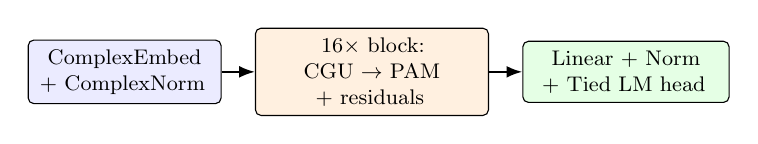
\begin{tikzpicture}[
      scale=0.85, transform shape,
      font=\small,
      box/.style={draw, rounded corners=2pt, minimum height=8mm, inner sep=4pt},
      arrow/.style={-{Latex[length=2mm]}, thick},
    ]
      \node[box, fill=blue!8, text width=2.6cm, align=center] (emb) {ComplexEmbed + ComplexNorm};
      \node[box, right=5mm of emb, fill=orange!12, text width=3.2cm, align=center] (block) {$16\times$ block:\\CGU $\to$ PAM\\+ residuals};
      \node[box, right=5mm of block, fill=green!10, text width=2.8cm, align=center] (head) {Linear + Norm + Tied LM head};
      \draw[arrow] (emb) -- (block);
      \draw[arrow] (block) -- (head);
    \end{tikzpicture}
    \caption{\textbf{medium-pam-v3} backbone: interleaved channel mixing (CGU) and sequence mixing (PAM) per block.}
    \label{fig:arch-backbone}
  \end{subfigure}

  \vspace{0.8em}
  \begin{subfigure}[b]{\textwidth}
    \centering
    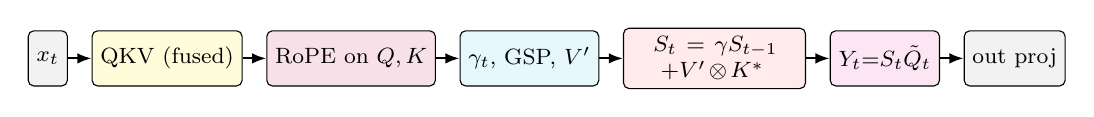
\begin{tikzpicture}[
      font=\footnotesize,
      box/.style={draw, rounded corners=2pt, minimum height=7mm, inner sep=3pt},
      arrow/.style={-{Latex[length=1.8mm]}, thick},
    ]
      \node[box, fill=gray!10] (in) {$x_t$};
      \node[box, right=3mm of in, fill=yellow!15] (qkv) {QKV (fused)};
      \node[box, right=3mm of qkv, fill=purple!12] (rope) {RoPE on $Q,K$};
      \node[box, right=3mm of rope, fill=cyan!10] (g) {$\gamma_t$, GSP, $V'$};
      \node[box, right=3mm of g, fill=red!8, text width=2.1cm, align=center] (S) {$S_t = \gamma S_{t-1}$\\$+ V'\!\otimes\! K^*$};
      \node[box, right=3mm of S, fill=magenta!10] (y) {$Y_t{=}S_t \tilde{Q}_t$};
      \node[box, right=3mm of y, fill=gray!10] (out) {out proj};
      \draw[arrow] (in) -- (qkv);
      \draw[arrow] (qkv) -- (rope);
      \draw[arrow] (rope) -- (g);
      \draw[arrow] (g) -- (S);
      \draw[arrow] (S) -- (y);
      \draw[arrow] (y) -- (out);
    \end{tikzpicture}
    \caption{Single PAM head (inference path): fused QKV, complex RoPE on $Q,K$, decay and GSP, outer-product write to matrix state, retrieval with scaled query $\tilde{Q}_t=Q_t/\sqrt{d}$, output projection.}
    \label{fig:arch-pam}
  \end{subfigure}
  \caption{Architecture diagrams for Phase-Associative Memory (\textbf{medium-pam-v3}).}
  \label{fig:architecture}
\end{figure}

\section{Experimental Setup}
\label{sec:exp}

\subsection{Dataset}
We train and evaluate on WikiText-103~\cite{merity2017pointer}, a standard language modeling benchmark containing approximately 103 million tokens of Wikipedia text. We use the official train/validation splits, tokenized with the GPT-2 BPE tokenizer (vocabulary size 50,257).

\subsection{Model configuration}
\textbf{Primary reported model (medium-pam-v3).} See \cref{tab:config}.

\begin{table}[t]
  \centering
  \caption{medium-pam-v3 configuration (reported).}
  \label{tab:config}
  \begin{tabular}{@{}ll@{}}
    \toprule
    Parameter & Value \\
    \midrule
    Complex dimension ($D$) & 384 \\
    Blocks & 16 (each: CGU $\to$ PAM) \\
    Interleave CGU + PAM & yes (\texttt{interleave\_pam=True}) \\
    CGU expansion factor & 3 \\
    PAM heads ($H$) & 6 \\
    PAM head dimension ($d$) & 64 \\
    GSP & enabled \\
    PAM RoPE on $Q, K$ & yes (\texttt{pam\_rope=True}) \\
    PAM QK phase norm & \textbf{off} (\texttt{pam\_qk\_norm=False}; see \cref{sec:main-result}) \\
    Fused QKV projection & yes (\texttt{pam\_fused\_qkv=True}) \\
    Sequence length & 2048 \\
    Total parameters & $\sim$100.4M \\
    Working/internal memory & disabled \\
    Softmax attention & disabled \\
    \bottomrule
  \end{tabular}
\end{table}

\subsection{Training details}
Hyperparameters below match \textbf{medium-pam-v3} (preset \texttt{medium-pam-v3} in \texttt{v6/config.py}). The earlier \textbf{sequential} \texttt{medium-pam} run used learning rate $3 \times 10^{-5}$ and 500 warmup steps (\cref{sec:main-result}).

\begin{table}[t]
  \centering
  \caption{Training hyperparameters (medium-pam-v3).}
  \label{tab:train}
  \begin{tabular}{@{}ll@{}}
    \toprule
    Parameter & Value \\
    \midrule
    Optimizer & AdamW \\
    Learning rate & $1 \times 10^{-4}$ \\
    Weight decay & 0.01 \\
    Warmup steps & 1000 \\
    LR schedule & warmup + cosine decay \\
    Batch size & 3 \\
    Epochs & 10 \\
    Gradient clipping & 1.0 \\
    Precision & automatic mixed precision (bf16) \\
    Hardware & single NVIDIA RTX 4090 (24GB) \\
    Compilation & torch.compile (default mode) \\
    Initialization & orthogonal (complex linear maps) \\
    \bottomrule
  \end{tabular}
\end{table}

\subsection{Generation settings (qualitative evaluation)}
During training, generation samples are logged every 5,000 steps using: temperature 1.0; top-$k$ 50; top-$p$ 0.9; repetition penalty 1.2.

\section{Results}
\label{sec:results}

\subsection{Main result}
\label{sec:main-result}
\textbf{medium-pam-v3} (interleaved + RoPE + fused QKV, no QK phase norm) reaches validation perplexity \textbf{29.95} after 10 epochs on WikiText-103 (single run, RTX 4090). \cref{fig:valppl,fig:train-snapshot,tab:mainppl} summarize training progress.

\begin{table}[t]
  \centering
  \caption{medium-pam-v3: training and validation perplexity by epoch (WikiText-103).}
  \label{tab:mainppl}
  \begin{tabular}{@{}rcc@{}}
    \toprule
    Epoch & Train PPL & Val PPL \\
    \midrule
    1 & 123.86 & 57.94 \\
    2 & 53.87 & 43.83 \\
    3 & 44.88 & 38.69 \\
    4 & 40.39 & 35.88 \\
    5 & 37.42 & 33.82 \\
    6 & 35.13 & 32.25 \\
    7 & 33.26 & 31.22 \\
    8 & 31.78 & 30.40 \\
    9 & 30.66 & 30.01 \\
    10 & 30.02 & \textbf{29.95} \\
    \bottomrule
  \end{tabular}
\end{table}

\begin{figure}[t]
  \centering
  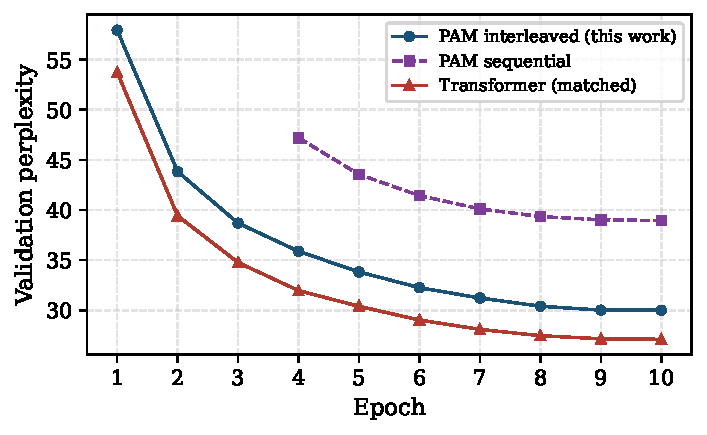
\includegraphics[width=0.72\linewidth]{figures/val_ppl_curve.pdf}
  \caption{Validation perplexity vs.\ epoch for \textbf{medium-pam-v3} (same data as \cref{tab:mainppl}).}
  \label{fig:valppl}
\end{figure}

\begin{figure}[t]
  \centering
  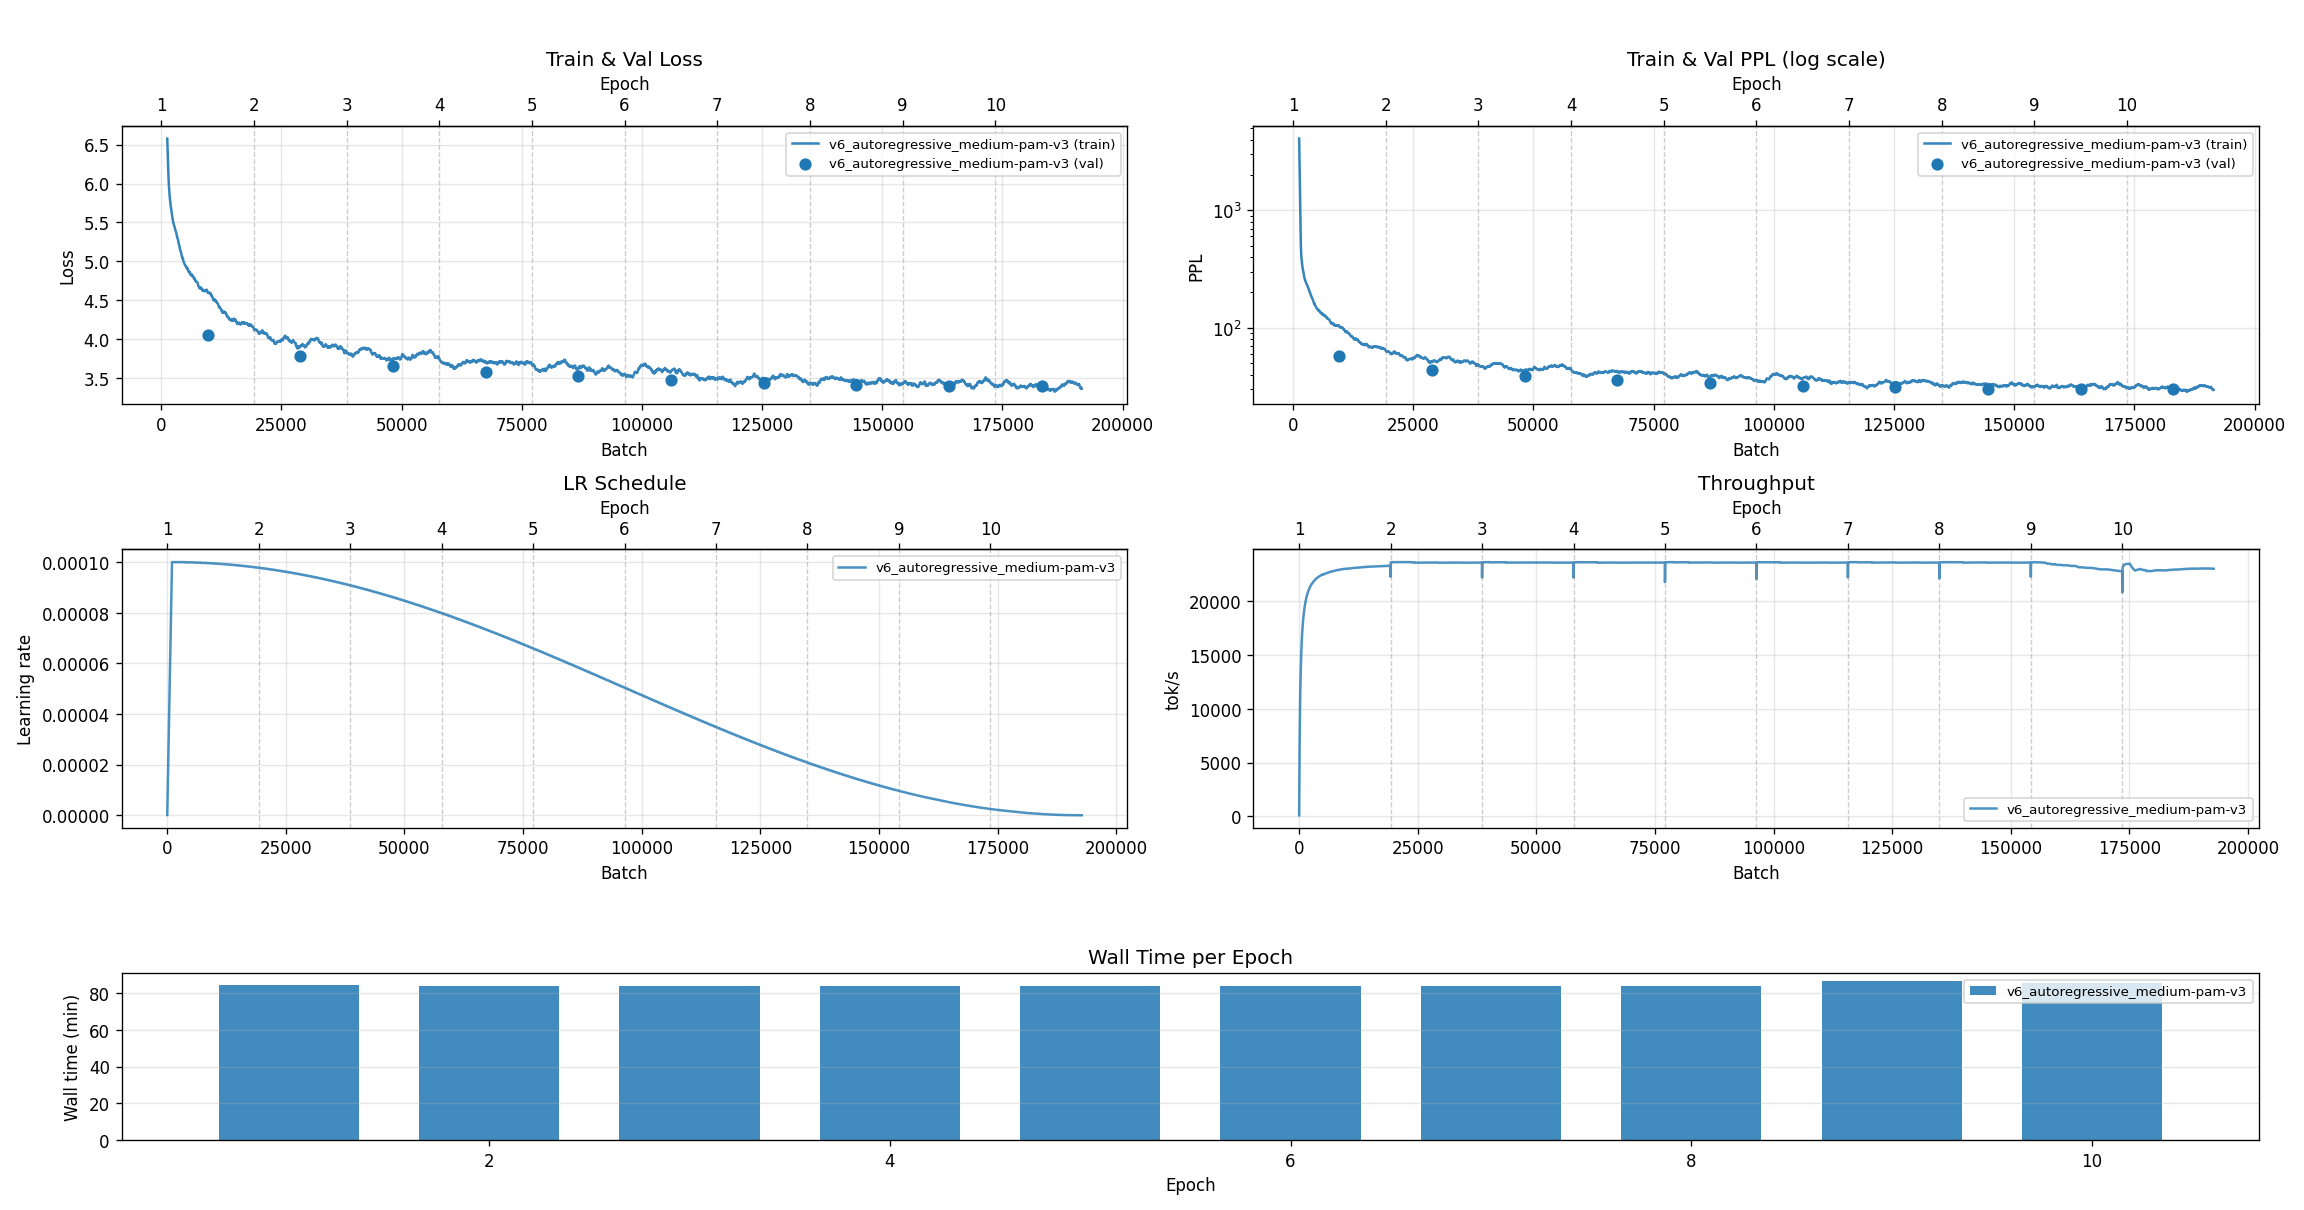
\includegraphics[width=\linewidth]{figures/training_run_medium_pam_v3.png}
  \caption{Live training monitor for the reported run (git \texttt{31397f0}; wall 50714.3~s; best val PPL \textbf{29.95}). Logs under \texttt{logs/v6/}\allowbreak\texttt{/medium\_pam\_v3\_rope\_wikitext103\_20260319\_231524\_31397f0/}.}
  \label{fig:train-snapshot}
\end{figure}

Total wall time \textbf{50,714 s ($\sim$14.1 h)}. Throughput \textbf{$\sim$23k tokens/second} average.

\paragraph{QK phase normalization ablation.} We briefly trained with per-element unit normalization of $Q$ and $K$ before the dot product. Validation loss decreased, but \textbf{generation} collapsed into severe lexical repetition by mid-training; we \textbf{stopped} the run during \textbf{epoch 5}. PAM scores are not softmax-normalized; removing $Q/K$ magnitude removes a degree of freedom that appears important for non-softmax retrieval. We \textbf{do not} use QK phase norm in the reported preset (see project log \texttt{EXPERIMENTS\_V6\_PART2.md}, Bug~8).

\paragraph{Earlier configuration: sequential medium-pam.} An earlier \textbf{sequential} stack (16 CGU layers then 16 PAM layers), no RoPE, learning rate $3 \times 10^{-5}$, 500 warmup steps, achieved \textbf{38.95} validation PPL after 10 epochs. Epochs 1--3 had correct PPL but a train/inference path bug affecting \textbf{generation} only; the run was resumed from the epoch 3 checkpoint with the fix. PPL for epochs 4--10 is shown in \cref{tab:seqppl}.

\begin{table}[t]
  \centering
  \caption{Sequential medium-pam: epochs 4--10 after resume (WikiText-103).}
  \label{tab:seqppl}
  \begin{tabular}{@{}rcc@{}}
    \toprule
    Epoch & Train PPL & Val PPL \\
    \midrule
    4 & 54.03 & 47.19 \\
    5 & 48.55 & 43.55 \\
    6 & 45.26 & 41.43 \\
    7 & 43.14 & 40.11 \\
    8 & 41.76 & 39.34 \\
    9 & 40.91 & 39.02 \\
    10 & 40.50 & \textbf{38.95} \\
    \bottomrule
  \end{tabular}
\end{table}

Wall time for that continuation was \textbf{$\sim$9.9 h}; throughput \textbf{$\sim$23,500 tok/s}.

The \textbf{29.95} vs \textbf{38.95} comparison is \textbf{not} a controlled ablation: layout, RoPE, fused QKV, block GEMM packaging, and \textbf{training hyperparameters} changed together.

\paragraph{Hybrid PAM + sparse attention (PIA).} We tested \textbf{medium-pam-v3-pia}, which adds Phase Interference Attention (PIA)---a windowed ($w{=}256$), sparse attention layer inserted every 4th block---on top of the medium-pam-v3 architecture. This hybrid achieved \textbf{30.01} validation PPL, marginally \textbf{worse} than pure PAM (29.95), while increasing wall time to 16.4~h ($\sim$20k tok/s). The result suggests that PAM's recurrent sequence mixing already captures the information that sparse attention would provide at this scale, and the added complexity does not help.

\subsection{Ablation across V6 architectures}
\label{sec:ablation}
\cref{tab:v6prog} shows the progression of V6 architectures on WikiText-103 (10 epochs, sequence length 2048 where noted). Rows are \textbf{not} a single-variable grid.

\begin{table}[t]
  \centering
  \caption{V6 architecture progression on WikiText-103 (validation perplexity). The transformer baseline uses the same data, tokenizer, sequence length, and training budget.}
  \label{tab:v6prog}
  \begin{tabular}{@{}>{\raggedright\arraybackslash}p{2.4cm} >{\raggedright\arraybackslash}p{5.4cm} cc@{}}
    \toprule
    Model & Architecture & Params & Val PPL \\
    \midrule
    medium-rebalanced & CGU + vector-state SSM & 58.4M & 44.47 \\
    medium-rebalanced-gsp & CGU + SSM + GSP & 63.2M & 41.67 \\
    medium-rebalanced-hsb & CGU + SSM + GSP + HSB & 75.0M & 43.54 \\
    medium-pam & CGU $\times$16 then PAM $\times$16 + GSP & 100.4M & 38.95 \\
    medium-pam-v3-pia & medium-pam-v3 + sparse PIA (every 4 blocks) & $\sim$100.4M & 30.01 \\
    \textbf{medium-pam-v3} & \textbf{16$\times$[CGU$\to$PAM] + GSP + RoPE + fused QKV} & \textbf{$\sim$100.4M} & \textbf{29.95} \\
    \midrule
    Transformer (ours) & Standard transformer (12 layers, 12 heads) & $\sim$100.3M & 27.08 \\
    \bottomrule
  \end{tabular}
\end{table}

Key observations:
\begin{itemize}
  \item \textbf{GSP helps}: Adding Gated State Protection to the SSM baseline reduces perplexity from 44.47 to 41.67 (6.3\% improvement).
  \item \textbf{HSB hurts}: Holographic State Binding causes a regression to 43.54. This supports the interference hypothesis: vector states lack capacity for multiple simultaneous associations.
  \item \textbf{PAM works}: Matrix-state PAM improves over the GSP SSM baseline; \textbf{medium-pam-v3} further improves over sequential \textbf{medium-pam} (layout + RoPE + recipe), reaching \textbf{29.95}.
  \item \textbf{PIA adds no benefit}: Adding sparse Phase Interference Attention (windowed, every 4th block) to medium-pam-v3 yields 30.01, marginally \textbf{worse} than pure PAM (29.95). PAM's sequence mixing appears sufficient without supplemental attention.
  \item \textbf{Transformer gap}: A matched transformer baseline reaches \textbf{27.08}, a $\sim$10\% advantage over medium-pam-v3. See \cref{sec:transformer-comparison} for detailed analysis.
\end{itemize}

\subsection{Comparison to matched transformer baseline}
\label{sec:transformer-comparison}
To provide a rigorous comparison, we trained a standard transformer with $\sim$100.3M parameters on the same WikiText-103 data, tokenizer (GPT-2 BPE), sequence length (2048), batch size (3), learning rate ($1 \times 10^{-4}$), warmup (1000 steps), and hardware (single RTX 4090). The transformer uses $d_{\text{model}} = 672$, 12 layers, 12 attention heads, and $d_{\text{ff}} = 2688$.

\begin{table}[t]
  \centering
  \caption{Matched comparison: transformer baseline vs.\ PAM (same data, tokenizer, seq\_len, LR, hardware).}
  \label{tab:gpt2}
  \begin{tabular}{@{}lccccc@{}}
    \toprule
    Model & Type & Params & Val PPL & Wall time & Throughput \\
    \midrule
    GPT-2 (cited) & Transformer & 124M & $\sim$31 & -- & -- \\
    Transformer (ours) & Transformer & $\sim$100.3M & \textbf{27.08} & 3.5~h & $\sim$96k tok/s \\
    \textbf{PAM (ours)} & \textbf{Complex recurrent} & \textbf{$\sim$100.4M} & \textbf{29.95} & \textbf{14.1~h} & \textbf{$\sim$23k tok/s} \\
    \bottomrule
  \end{tabular}
\end{table}

\textbf{medium-pam-v3} reaches \textbf{29.95} validation PPL vs.\ the matched transformer's \textbf{27.08}---a gap of $\sim$10\%. The transformer also trains $\sim$4$\times$ faster in wall time (3.5~h vs.\ 14.1~h) and throughput ($\sim$96k vs.\ $\sim$23k tok/s). The throughput gap is expected: complex linear maps require 4$\times$ the multiply-adds of real linear maps, and PAM uses pure PyTorch with no custom kernels.

For external reference, the commonly cited GPT-2~\cite{radford2019language} validation PPL on WikiText-103 is $\sim$31 at 124M parameters (test PPL $\sim$14.84 uses a different sliding-window protocol and is not directly comparable).

\begin{table}[t]
  \centering
  \caption{Epoch-by-epoch validation PPL: matched transformer vs.\ medium-pam-v3.}
  \label{tab:epoch-comparison}
  \begin{tabular}{@{}rccccc@{}}
    \toprule
    & \multicolumn{2}{c}{Transformer (ours)} & & \multicolumn{2}{c}{PAM (ours)} \\
    \cmidrule{2-3} \cmidrule{5-6}
    Epoch & Train PPL & Val PPL & & Train PPL & Val PPL \\
    \midrule
    1 & 137.77 & 53.74 & & 123.86 & 57.94 \\
    2 & 52.81 & 39.42 & & 53.87 & 43.83 \\
    3 & 42.74 & 34.76 & & 44.88 & 38.69 \\
    4 & 38.27 & 31.96 & & 40.39 & 35.88 \\
    5 & 35.54 & 30.39 & & 37.42 & 33.82 \\
    6 & 33.41 & 29.02 & & 35.13 & 32.25 \\
    7 & 31.65 & 28.09 & & 33.26 & 31.22 \\
    8 & 30.28 & 27.46 & & 31.78 & 30.40 \\
    9 & 29.29 & 27.15 & & 30.66 & 30.01 \\
    10 & 28.75 & \textbf{27.08} & & 30.02 & \textbf{29.95} \\
    \bottomrule
  \end{tabular}
\end{table}

The transformer converges faster and maintains a consistent advantage throughout training (\cref{tab:epoch-comparison}). Both models use the same epoch count and see the same total tokens.

Structural differences remain important despite the PPL gap:
\begin{itemize}
  \item \textbf{Inference cost}: The transformer requires $O(T)$ work per token (KV cache); PAM is $O(1)$ per token with fixed-size state (per-layer work $O(Hd^2)$, independent of sequence length).
  \item \textbf{Memory footprint}: The transformer's KV cache grows linearly with sequence length; PAM's state is fixed at 49,152 floats per layer regardless of $T$.
  \item \textbf{Architecture maturity}: Transformers benefit from years of optimization (FlashAttention, fused kernels, etc.); PAM is a first-generation PyTorch implementation with no custom CUDA kernels.
\end{itemize}

\subsection{Generation quality}
\textbf{medium-pam-v3 (epoch 10)} produces coherent multi-sentence text; factual accuracy is not guaranteed.

\paragraph{Prompt:} \texttt{In 1923 , the University of}

\paragraph{Generated text (medium-pam-v3, epoch 10):}
\begin{quote}
In 1923 , the University of Illinois at Urbana @-@ Urdu said it was " an easy choice to do something in its own right . " The university also claimed the first students from Wisconsin had to be replaced by a more " good student " due to a lack of funds .
\end{quote}

Quality metrics at final epoch: 3-gram repetition rate \textbf{0.034}, 4-gram repetition rate \textbf{0.011}, zero restarts, unique token ratio \textbf{0.703}. The sample shows section-like structure and WikiText-style tokenization artifacts; it does \textbf{not} exhibit the list-repetition failure mode of the QK-norm ablation.

\paragraph{Sequential medium-pam (epoch 10)} for the same prompt (different run, see \cref{sec:main-result}):
\begin{quote}
In 1923 , the University of Missouri and the University of Michigan was also established in 1926 . In 1928 , the University of Michigan opened its current campus with the school 's first campus opening at St. Louis Road on the northern end of Lake Michigan in 1929 .
\end{quote}

Quality metrics (sequential run): 3-gram rep.\ 0.051, 4-gram rep.\ 0.020, unique token ratio 0.624.

The text is grammatically coherent and shows structural awareness (dates, proper nouns, institutional language). Factual accuracy is not reliable---this is expected at this scale.

\subsection{Earlier validation: TinyStories}
Before WikiText-103, the broader V6 architecture family was validated on TinyStories~\cite{eldan2023tinystories}:
\begin{table}[h]
  \centering
  \begin{tabular}{@{}llccc@{}}
    \toprule
    Model & Config & Params & Dataset & Val PPL \\
    \midrule
    V6 small-matched & CGU + SSM, no memory & 28.7M & TinyStories (full) & 5.50 \\
    V6 small-matched & CGU + SSM, WM=16 & 29.2M & TinyStories (full) & 2.23 \\
    \bottomrule
  \end{tabular}
\end{table}

These results established that the phase-preserving, attention-free architecture family can learn effectively. The TinyStories experiments also revealed that working memory capacity is a critical control variable: too much memory induces memorization, while zero memory produces cleaner but higher-perplexity generations.

\section{Analysis}
\label{sec:analysis}

\subsection{Why HSB failed and PAM works}
\label{sec:hsb}
The progression from SSM to HSB to PAM illustrates a specific failure mode and its solution.

\textbf{Holographic State Binding (HSB)} attempted to inject key--value associations into the SSM's vector state using complex multiplication (the HRR binding operation). Mathematically, multiple bindings are superposed additively in the same $d$-dimensional vector. When only a few associations are present, retrieval via conjugate multiplication works. When many associations accumulate over a long sequence, they interfere destructively---the signal-to-noise ratio is often discussed heuristically as degrading with the number of superposed associations in HRR-style models (e.g.\ as $O(1/\sqrt{n})$ scaling in classical analyses of superposition).

\textbf{PAM} solves this by replacing the vector state with a matrix state. The outer product $V_t \otimes K_t^*$ writes each association into a separate subspace of the $d \times d$ matrix. Multiple associations can coexist without interfering because they occupy different rank-1 components of the matrix. The capacity is $O(d^2)$ per head rather than $O(d)$.

This diagnosis---vector state causes interference, matrix state fixes it---is supported by the experimental evidence: HSB regresses from the SSM baseline, while PAM improves over it.

\subsection{Phase interference as implicit attention}
In standard attention, the softmax over $QK^\top / \sqrt{d}$ produces a probability distribution that weights values. In PAM, the complex dot product $K_i^* \cdot \tilde{Q}_t$ serves an analogous role:
\begin{align}
  \text{Attention: } \alpha_{ti} &= \frac{\exp(Q_t \cdot K_i / \sqrt{d})}{\sum_j \exp(Q_t \cdot K_j / \sqrt{d})} \\
  \text{PAM: } w_{ti} &= \left(\prod_{j=i+1}^{t} \gamma_j\right) \cdot (K_i^* \cdot \tilde{Q}_t) .
\end{align}
The key differences:
\begin{enumerate}
  \item PAM weights are \textbf{complex-valued}, not positive real. This means retrieval can involve both addition and cancellation, potentially providing richer composition.
  \item PAM weights are \textbf{not normalized}. There is no softmax or equivalent. This removes a nonlinearity but also removes the guarantee that weights sum to 1.
  \item PAM weights include a \textbf{decay factor} that naturally downweights distant positions, providing a soft locality bias that attention must learn.
  \item PAM weights depend on \textbf{phase alignment}, a geometric property of complex vectors that standard real-valued attention lacks.
\end{enumerate}
Whether these differences are advantageous at scale is an open question. The current evidence is that they produce a trainable system with reasonable perplexity, but we cannot yet determine whether phase interference provides benefits beyond what real-valued matrix states achieve.

\subsection{Computational cost}
\textbf{Training}: The dual form computes $W = \tilde{Q} K^{*\top}$ (after RoPE on $Q,K$) as a $T \times T$ matrix per head, giving $O(T^2 H d)$ cost per layer---the same order as standard attention. For $T = 2048$, this is efficient on modern GPUs. \textbf{medium-pam-v3} training throughput is approximately \textbf{23k tokens/second} on a single RTX 4090 (wall time \textbf{$\sim$14.1 h} for 10 epochs). By comparison, our matched transformer baseline achieves $\sim$\textbf{96k tokens/second} (wall time $\sim$3.5~h), a $\sim$4$\times$ throughput advantage. This gap is expected: complex linear maps require 4$\times$ the multiply-adds of real linear maps, and the PAM implementation uses no custom CUDA kernels.

\textbf{Inference}: The recurrent form processes each token with $O(Hd^2)$ work per layer (one matrix--vector multiply per head). With $H = 6$ and $d = 64$, this is 24,576 complex multiply-adds per layer. The state is $H \times d \times d \times 2$ floats $= 6 \times 64 \times 64 \times 2 = 49{,}152$ floats per layer, regardless of sequence length.

For comparison, a transformer's KV cache stores $2 \times H \times d \times T$ values per layer, growing linearly with $T$. At $T = 2048$ with our baseline's configuration ($H{=}12$, $d{=}56$), the cache per layer is $2 \times 12 \times 56 \times 2048 = 2{,}752{,}512$ values. PAM's state per layer is fixed at 49,152 values, a factor of $\sim$56$\times$ smaller at this sequence length, and the advantage grows with longer sequences.

\subsection{The role of GSP}
GSP's protect gate allows the model to selectively override decay, retaining specific state dimensions indefinitely. This is conceptually similar to the forget gate in LSTMs but operates at the level of the entire $d \times d$ state matrix per head. Empirically, GSP improves the SSM baseline from 44.47 to 41.67 perplexity, and PAM uses GSP by default.

The protect gate also modulates the value signal ($V' = V \cdot (1 - p)$), preventing new values from overwriting protected dimensions. This creates a natural partitioning of state into ``active'' dimensions (low protection, normal read/write) and ``frozen'' dimensions (high protection, retained over long spans).

\section{Limitations}
All results in this paper (PAM and the matched transformer baseline) come from \textbf{single} training runs. We have not measured variance across seeds or conducted full architecture search. The $\sim$10\% gap between PAM (29.95) and the matched transformer (27.08) should be interpreted with this caveat.

100M parameters and WikiText-103 are modest by current standards. We do not know how PAM scales to billions of parameters or web-scale corpora. The $O(d^2)$ state per head could become a memory concern at very large head dimensions, though for the current $d = 64$ it is negligible.

We report perplexity and qualitative generation only. Standard downstream benchmarks (LAMBADA, HellaSwag, etc.) have not been evaluated.

PAM is implemented in pure PyTorch with no custom CUDA kernels. The dual form uses standard matrix multiplications, which are efficient, but the recurrent form's sequential loop is not optimized. Custom kernels for the state update and retrieval could improve inference throughput substantially.

Complex linear maps require 4$\times$ the multiply-adds of real linear maps. The reference implementation is equivalent to four real matrix multiplies; \textbf{training} uses a \textbf{block-real GEMM} that is numerically equivalent (max float32 diff $\sim 4\times 10^{-6}$ in our checks). Whether the representational advantages of complex computation compensate for this overhead at scale is unresolved.

The V6 codebase includes working memory, internal memory, persistent memory, expert memory, and session memory modules. The \textbf{medium-pam-v3} run reported here disables all of these (no working memory, no internal memory) to isolate PAM's contribution. Whether combining PAM with memory modules improves results is an open question.

\section{Future Work}
At 100M parameters, our matched transformer baseline outperforms PAM by $\sim$10\% on validation PPL. The most immediate scaling question is whether this gap widens, narrows, or holds at larger scales. We plan to train larger PAM models (300M--1B parameters) alongside matched transformer baselines on the same data and compute budget.

The recurrent inference form's sequential loop is a clear optimization target. A fused CUDA kernel for the complex matrix state update and retrieval could bring PAM's wall-clock inference speed closer to its theoretical advantage.

PAM's fixed-size state and absence of KV cache make it theoretically well-suited for long sequences. We plan to evaluate on PG-19 and other long-document benchmarks to test whether the $O(d^2)$ state capacity is sufficient for practical long-context modeling.

The V6 codebase includes a memory hierarchy (working, internal, persistent, expert) with phase-coherence retrieval. These modules were disabled for the PAM evaluation to isolate the core contribution. Integrating PAM with working memory and evaluating on tasks that require explicit fact storage is a natural next step.

PAM could be combined with sparse attention layers to create a hybrid architecture. Our initial experiment with PIA (Phase Interference Attention, windowed, every 4th block) showed no improvement over pure PAM at this scale (\cref{sec:ablation}). However, alternative hybrid strategies---such as full (non-windowed) attention at select layers, or standard softmax attention rather than phase-based---remain unexplored.

\paragraph{Prior hybrid (V5 lineage).} \textbf{In this research line}, the earlier \textbf{V5} codebase first combined end-to-end phase-preserving complex sequence modeling with \textbf{sparse} PhaseAttention (sliding window, every $K$ layers) and trained it to strong TinyStories perplexity, establishing a working complex-phase--limited-attention stack before the attention-free PAM direction (see \texttt{v5/EXPERIMENTS.md}).

The shared backbone design in V6 was built to support both autoregressive and diffusion modes on the same architecture. Extending PAM to image generation or multimodal modeling is architecturally straightforward but experimentally unvalidated.

\section{Conclusion}

The central finding of this work is that complex-valued phase interference---constructive and destructive, arising from the conjugate inner product between queries and stored keys---is sufficient for competitive sequence modeling. At $\sim$100M parameters on WikiText-103, PAM achieves validation perplexity \textbf{29.95}, within $\sim$10\% of a matched transformer baseline (\textbf{27.08}) trained under identical conditions. The gap was achieved without custom CUDA kernels and with 4$\times$ arithmetic overhead from complex computation. We do not claim parity with transformers. What we do claim is that the gap is small enough, given these handicaps, to constitute evidence that the algebraic structure of complex interference is well-matched to the problem of sequence modeling---and that this match is worth investigating further.

The progression from vector-state SSMs (interference-limited, with holographic binding degrading as $O(1/\sqrt{n})$) to matrix-state PAM ($O(d^2)$ capacity per head) illustrates a specific failure mode and its resolution. The further improvement from sequential to interleaved layout with complex RoPE demonstrates that standard architectural principles (alternating channel and sequence mixing, relative position encoding) transfer cleanly to complex-valued computation. These are engineering results. But the deeper question---why complex-valued phase interference works for language at all---connects to the empirical evidence that semantic interpretation exhibits non-classical contextuality~\cite{agostino2025quantum,agostino2026production,busemeyer2012quantum}. If meanings are produced through interference between possible interpretations rather than retrieved from a fixed store, then an architecture whose native operations are superposition and phase-dependent retrieval may be capturing something about the structure of the problem that real-valued architectures must learn indirectly. Whether this structural consonance has practical consequences at scale---whether phase provides an inductive bias that narrows or widens the gap as models grow---is the most important open question this work raises, and the one we intend to pursue.

\appendix

\section{Hyperparameter Details}
\subsection{medium-pam-v3 configuration (reported)}
\begin{verbatim}
preset:               medium-pam-v3
vocab_size:           50,257
complex_dim:          384
num_layers:           16
single_bank:          True
bank_expand:          3 (CGU hidden = 1,152)
interleave_pam:       True
state_dim:            0 (SSM disabled)
pam_num_heads:        6
pam_head_dim:         64
pam_rope:             True
pam_qk_norm:          False
pam_fused_qkv:        True
gated_state_protection: True
dropout:              0.1
init_strategy:        orthogonal
\end{verbatim}

\subsection{medium-pam configuration (sequential baseline)}
Same embedding and PAM head dimensions as above, but \textbf{no} interleaving, \textbf{no} RoPE, \textbf{no} fused QKV flag in the preset; training used \textbf{learning rate} $3 \times 10^{-5}$ and \textbf{500} warmup steps (see \cref{sec:main-result}). Full preset: \texttt{medium-pam} in \texttt{v6/config.py}.

\subsection{Matched transformer baseline configuration}
\begin{verbatim}
d_model:              672
n_layers:             12
n_heads:              12
d_ff:                 2688
total_parameters:     ~100.3M
dataset:              WikiText-103
tokenizer:            GPT-2 BPE (50,257 tokens)
seq_len:              2,048
batch_size:           3
optimizer:            AdamW
learning_rate:        1e-4
weight_decay:         0.01
warmup_steps:         1000
lr_schedule:          warmup + cosine decay
gradient_clip:        1.0
amp_dtype:            bf16 (automatic)
compile:              torch.compile (default mode)
hardware:             1x NVIDIA RTX 4090 (24GB)
\end{verbatim}

\subsection{Training configuration (medium-pam-v3)}
\begin{verbatim}
dataset:              WikiText-103
tokenizer:            GPT-2 BPE (50,257 tokens)
seq_len:              2,048
batch_size:           3
epochs:               10
optimizer:            AdamW
learning_rate:        1e-4
weight_decay:         0.01
warmup_steps:         1000
lr_schedule:          warmup + cosine decay
gradient_clip:        1.0
amp_dtype:            bf16 (automatic)
compile:              torch.compile (default mode)
hardware:             1x NVIDIA RTX 4090 (24GB)
\end{verbatim}

\subsection{Parameter breakdown}
\begin{table}[h]
  \centering
  \begin{tabular}{@{}lcc@{}}
    \toprule
    Component & Parameters & Percentage \\
    \midrule
    Embedding (tied with output) & $\sim$38.6M & 38.4\% \\
    CGU + PAM blocks (16 blocks) & $\sim$61.7M & 61.3\% \\
    LM head projection + norm & $\sim$0.3M & 0.3\% \\
    \textbf{Total} & \textbf{$\sim$100.4M} & \textbf{100\%} \\
    \bottomrule
  \end{tabular}
\end{table}

Note: the embedding accounts for a large fraction because dim=384 with vocab\_size=50,257 requires $50{,}257 \times 384 \times 2 = 38.6$M parameters (real + imaginary embedding tables). These are tied with the output layer.

\section{Reproducibility}
Full source code and training scripts: \url{https://github.com/gowrav-vishwakarma/qllm2}.

Python 3.9+ (tested with 3.9.24); PyTorch 2.x with CUDA support; package management via \texttt{uv}.

The reported \textbf{29.95} validation PPL run is archived under \texttt{logs/v6/medium\_pam\_v3\_rope\_wikitext103\_20260319\_231524\_31397f0/} (\texttt{RUN\_INFO.txt} lists git commit \texttt{31397f0} and full CLI). The matched transformer baseline (\textbf{27.08}) is archived under \texttt{logs/v6/transformer\_baseline\_wikitext103\_20260323\_140351\_e87b8e4/} (git commit \texttt{e87b8e4}).

\begin{verbatim}
uv sync && uv sync --extra cuda
./scripts/run_v6_medium_pam_v3.sh
./scripts/run_v6_medium_pam.sh
./scripts/run_v6_medium_pam.sh --resume
\end{verbatim}

Generation:
\begin{verbatim}
python -m v6.generate \
  --checkpoint checkpoints_v6_medium_pam_v3/best_model.pt \
  --prompt "In 1923 , the University of"
\end{verbatim}

\bibliographystyle{plainnat}
\bibliography{references}

\end{document}
